\documentclass[ignorenonframetext,mathserif]{beamer} %
%\usepackage[small]{eulervm}

\usepackage{amsmath}
\usepackage{amsfonts}

% \usepackage[english]{babel}
% \usepackage[latin1]{inputenc}
% \usepackage{times}
% \usepackage[T1]{fontenc}
% %\usepackage{rtsched}
\usepackage{graphicx}
% \usepackage{xmpmulti}
\usepackage{psfrag}
% \usepackage{listings}
% \usepackage{pst-node}
% \usepackage{amsmath}
% %\usepackage{grlist}
% %\usepackage{beamercode}
%\usepackage{pgfpages}
\usepackage{url}

\newcommand{\partder}[2]{\frac{\partial #1}{\partial #2}}
\newcommand{\eqdef}{\stackrel{\mbox{\tiny{\rm def}}}{=}}
\newcommand{\R}{\mathbb{R}}
\newcommand{\N}{\mathbb{N}}
\newcommand{\ud}{\mathrm{d}}
\newcommand{\dA}{\bar A}
\newcommand{\dB}{\bar B}
\newcommand{\dQ}{\bar Q}
\newcommand{\dR}{\bar R}
\newcommand{\dS}{\bar S}
\newcommand{\dP}{\bar P}
\newcommand{\dK}{\bar K}
\newcommand{\dW}{\bar W}

\newtheorem{proofsk}{Proof sketch}

\setbeamertemplate{navigation symbols}{} 

% \mode<handout>
% {
% \pgfpagesuselayout{2 on 1}[a4paper, border shrink=5mm]

% \setbeamercolor{background canvas}{bg=black!5}
% }

\mode<presentation>
{
  % \usetheme{CEIICP}
  %\usetheme{Warsaw}
%  \usetheme{Hannover}   % menu albero, semplice, titolo allineato a destra
%   %\usetheme{AnnArbor}   % giallo blu, troppo giallo?, niente menù mi sembra
%   %\usetheme{Antibes}    % Nero blu, struttura, troppo spazio rubato in alto
%   %\usetheme{Bergen}
%\usetheme{Berkeley}   % Blu, menu' albero con bar a sinistra, semplice
   %\usetheme{Berlin}     % varie tonalità blu a fasce, ben bilanciato
\usetheme{Boadilla}
%   %\usetheme{boxes}
%   %\usetheme{CambridgeUS}
%   %\usetheme{Copenhagen}
%   %\usetheme{Darmstadt}
%   %\usetheme{default}    % plain, con sfondo bianco
%   %\usetheme{Dresden}
%   %\usetheme{Frankfurt}
%   %\usetheme{Goettingen}
%   %\usetheme{Ilmenau}
%   %\usetheme{JuanLesPins}
%   %\usetheme{Luebeck}
%   %\usetheme{Madrid}
%   %\usetheme{Malmoe}

   %\usecolortheme{dolphin}
%   %\usecolortheme{sidebartab}
%   %\usecolortheme{seagull}  
%   %\usecolortheme{wolverine}
%   %\usecolortheme{dove}
%   \usecolortheme{iw}
%   %\usefonttheme{serif}
%   \useinnertheme{rounded}
%   %\useinnertheme{circles}
%   %\useoutertheme{miniframes}
}

\title[Classification of RTSS papers]
{Open and collaborative classification of RTSS papers}


\subtitle{(an attempt)}


\author[E. Bini]{\textbf{Enrico Bini}}

\institute[UniTo, Torino, Italy]{University of Turin}

\date[RTOPS'19, 24/07/2019]{Real-Time Systems Open Problems Seminar\\
{\small (special edition @RTSS19 PC meeting)}\\ July 24th, 2019}


%\subject{Talks}
% Inserisce la seguente slide all'inizio di ogni subsection
% \AtBeginSubsection[]
% {
%   \begin{frame}<beamer>
%     \frametitle{Outline}
%     \tableofcontents[currentsection,currentsubsection]
%   \end{frame}
% }

%Inserisce la seguente slide all'inizio di ogni section
\AtBeginSection[]
{
  \begin{frame}<beamer>
    \frametitle{Outline}
    \tableofcontents[currentsection]
  \end{frame}
}


\begin{document}

\begin{frame}
  \titlepage
\end{frame}

% ABSTRACT

% Oftentimes we find ourselves describing to colleagues what the real-time systems community investigates about. Not an easy task since timing is affected by all layers of abstractions: from the architecture up to languages. Also, the aging of researchers tends to limit the scientific memory to (say) 10 or 20 years. This may lead to the well-known phenomenon of periodic "reinvention of the wheel".

% In this presentation, it will be illustrated an effort made to classify all real-time papers. Papers ever published at RTSS are used as hopefully representative sample of the research community interests. Believing that claiming the authorship of such an effort will be an obstacle to contributions, this work is made publicly available on github. Contributions are more than welcome. 


\section{Introduction}

\begin{frame}
  \frametitle{Motivation}
  \begin{itemize}
  \item Researchers are aging. So the scientific memory does
  \item Forgetting research is going to worsen (I think)
    \begin{itemize}
    \item Growing number of papers per year
    \item ``Publish or perish'' pressure reduces the care in paper
      writing, including review/study of existing research
    \end{itemize}
  \item (personal motivation) I decided to illustrate at my new
    department (in Turin) what real-time research is about
  \item Result: a classification of all RTSS papers from 1990 to 2015
  \end{itemize}
\end{frame}

\section{Classification of RTSS papers: results}


\begin{frame}
  \frametitle{Classification of RTSS papers: methodology}
  
  \begin{itemize}
  \item Assuming that RTSS papers are a representative sample of the
    research on real-time systems
  \item Exhaustive classification of all RTSS papers available on
    IEEExplore (from 1990 to 2015): 927 papers.  
  \item Took three full days of work
    \begin{enumerate}
    \item a number $n$ ($=17$) of topics was identified (personal
      choice)
    \item each (of the 927) paper $j$ was assigned a weight
      $w_{ij}\geq 0$ representing how much such paper $j$ is related
      to topic $i$
      \[
      \forall \text{ paper } j,\qquad\sum_i w_{ij}= 1
      \]
    \item Weights $w_{ij}$ were computed by
      \begin{itemize}
      \item reading the title: 60\% of papers
      \item reading the abstract: 35\%
      \item reading the paper: 5\%
      \end{itemize}
    \end{enumerate}
  \item Example
    \begin{itemize}
    \item Paper $j$=``XYZ'' by \dots was assigned:
    \item $i=\text{topic 1}$, $w_{ij}=X$
    \item $i=\text{topic 2}$, $w_{ij}=X$
    \end{itemize}
  \end{itemize}
\end{frame}


\begin{frame}
  \frametitle{Classification of RTSS papers: results}
  \begin{center}
    \psfrag{lab1}[Bl]{\small autom, avion, medic, mmedia}
    \psfrag{lab2}[Bl]{\small control, AI}
    \psfrag{lab3}[Bl]{\small mixed criticality}
    \psfrag{lab4}[Bl]{\small lang, specs}
    \psfrag{lab5}[Bl]{\small formal methods, verif}
    \psfrag{lab6}[Bl]{\small W, battery, J harvest}
    \psfrag{lab7}[Bl]{\small design, comb-opt, ILP}
    \psfrag{lab8}[Bl]{\small DB, data mgmt}
    \psfrag{lab9}[Bl]{\small WSN}
    \psfrag{labA}[Bl]{\small distrib, faults, sync, cloud}
    \psfrag{labB}[Bl]{\small QoS-resource mgmt}
    \psfrag{labC}[Bl]{\small multi-proc sched}
    \psfrag{labD}[Bl]{\small 1-proc sched}
    \psfrag{labE}[Bl]{\small networks}
    \psfrag{labF}[Bl]{\small OS, I/O, disk, mem, res-sharing}
    \psfrag{labG}[Bl]{\small WCET, compiler, measure, stoc}
    \psfrag{labH}[Bl]{\small HW support, GPUs}
    % \psfrag{lab5}[Bl]{\small W, battery, J harvest}
    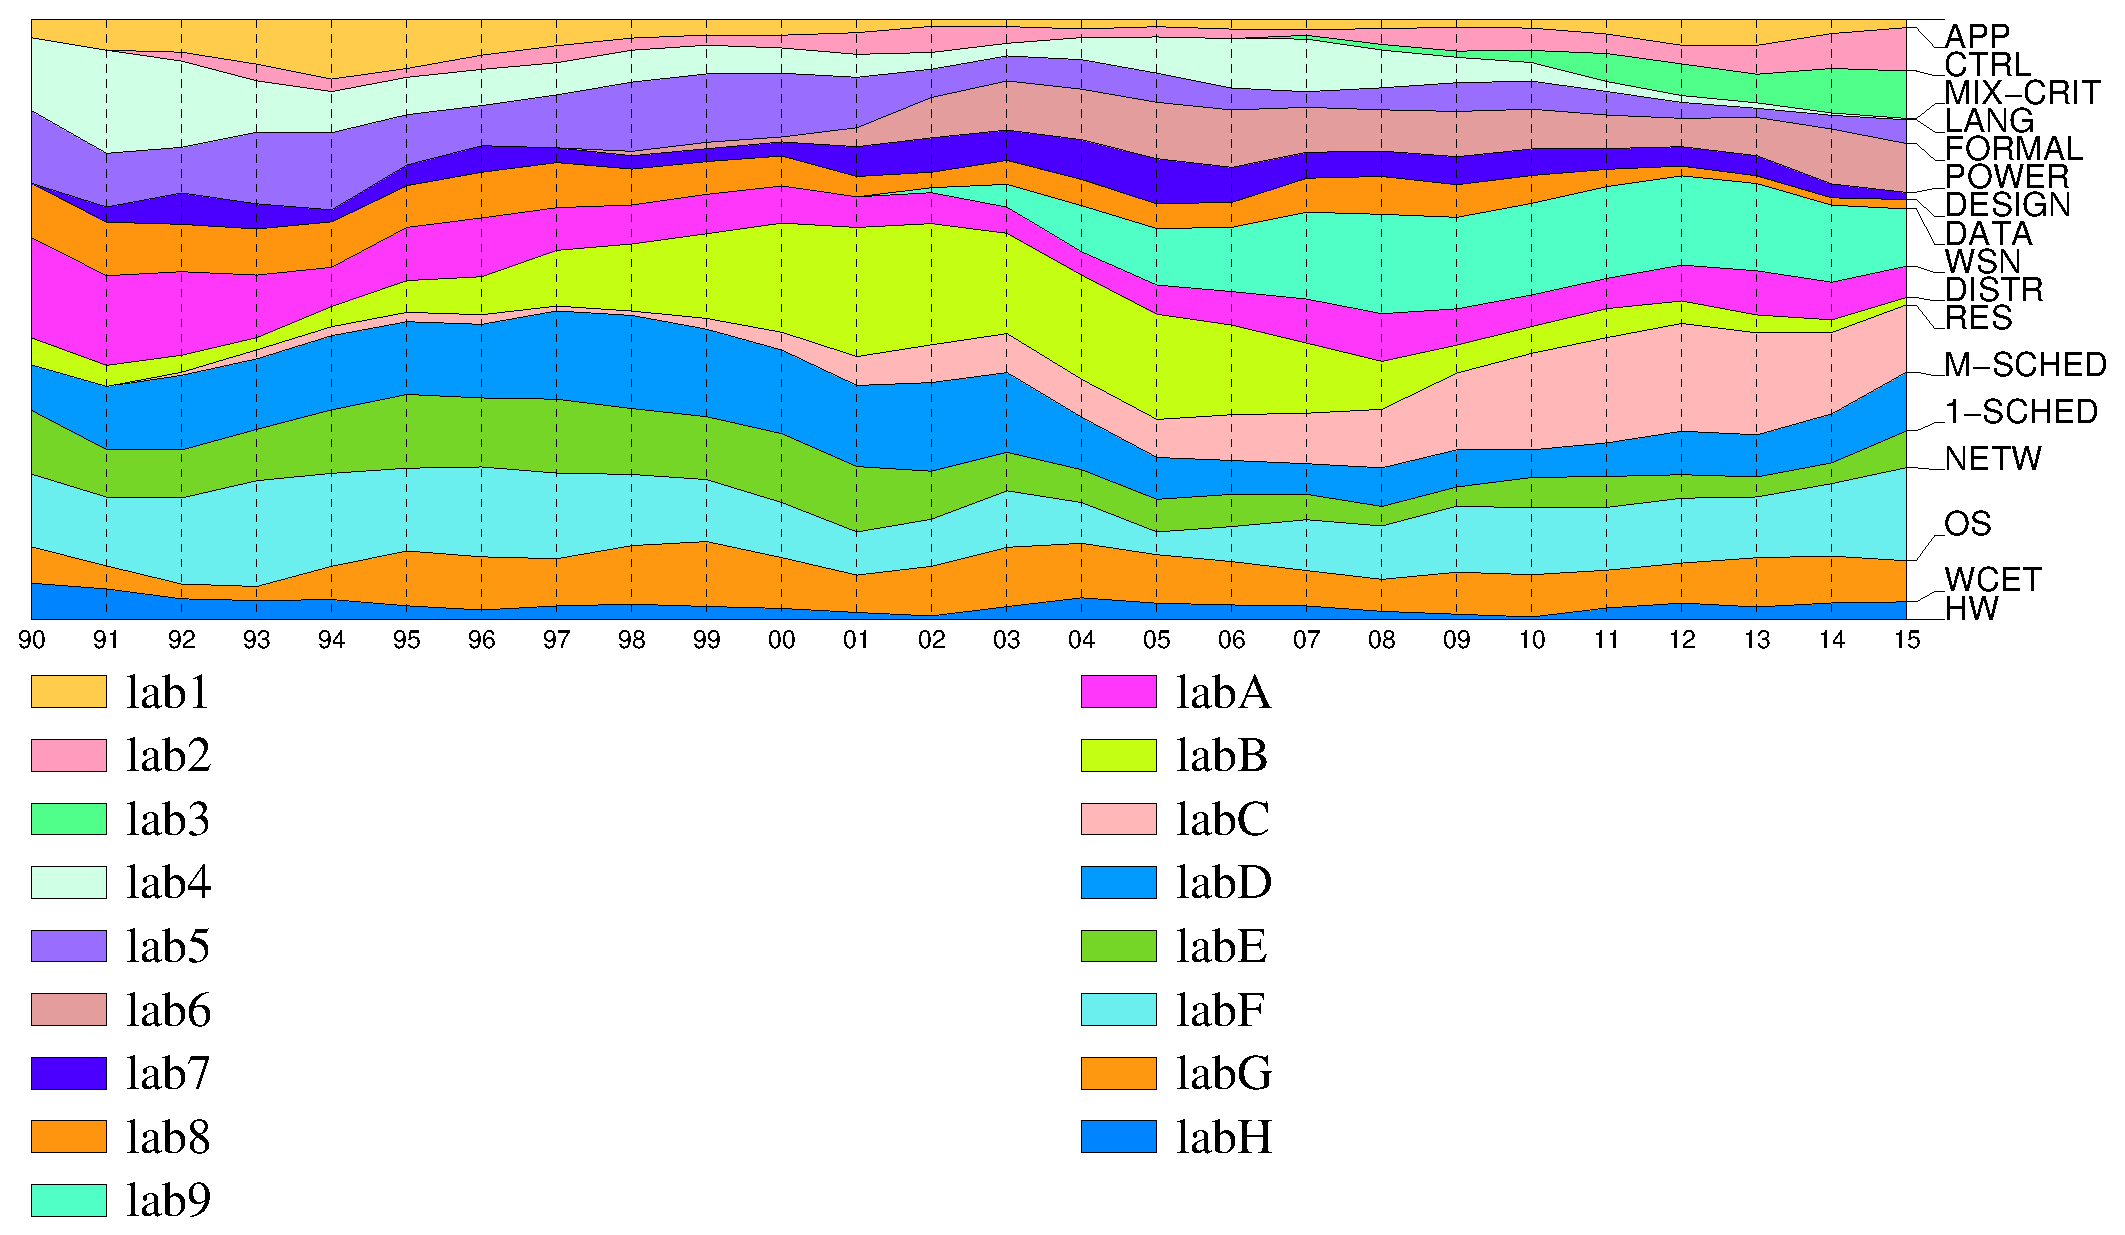
\includegraphics[scale=.34]{figs/topicsRT_2015}
  \end{center}

  % Mention the key names behind each topis: Jack Stankovic pushing
  % WSN and then Tarek Abdelzaher, Chenyang Lu
  % 
  % Strong group at UNC pushing both theoretical (Sanjoy Baruah) and
  % implementation-oriented (Jim Anderson) multiprocessor scheduling
  %
  % OS: strong group in Pisa, where we have developed the new Linux
  % scheduling class SCHED_DEADLINE as follow up of the EU project
  % ACTORS
  % 
  % Control: Lui Sha @UIUC, Karl-Erik Arzen Anton Cervin @Lund
  % 
  % Formal methods: Wang Yi @UppsalaU, Insup Lee @UPenn, Enrico
  % Vicario @unifi
  % 
  % recent trend on Mixed-Criticality: Burns @UnivOfYork

\end{frame}


\begin{frame}
  \frametitle{More methodology}
  \begin{itemize}
  \item sum of ``topics'' per year is computed (plot in next)
  \item data is filtered to smooth the trends
  \end{itemize}
\end{frame}
  

\begin{frame}[fragile]
  \frametitle{The status}

  \begin{itemize}
  \item Data is available on github:
    \begin{center}
      \url{https://github.com/ebni/classify-rt}
    \end{center}
    which you can get by
    \verb|git clone https://github.com/ebni/classify-rt.git|
  \item After chatting with Jim Anderson about this effort, he
    proposed me to publish the data on the IEEE TCRTS
  \end{itemize}
  \begin{center}
    \url{http://sites.ieee.org/tcrts/classification-of-rtss-papers/}
  \end{center}
  \begin{itemize}
  \item The repository contains:
    \begin{itemize}
    \item the raw data $w_{ij}$ paper data (\texttt{.csv} format) of
      2014, 2015
    \item the aggregate $\sum_{j\in\mathsf{paperPerYear}(y)}w_{ij}$
      per topic $i$ data of 1990--2013 (source $w_{ij}$ are probably
      lost)
    \item this presentation
    \end{itemize}
  \item Adding a new year requires:
    \begin{itemize}
    \item assign all $w_{ij}$ (about 2 hours depending)
    \item copy/paste data to some 
    \end{itemize}
  \end{itemize}
\end{frame}

\section{Future}

\begin{frame}
  \frametitle{Possible contributions (welcome)}
  \begin{itemize}
  \item Inserting the data for any new paper
  \item Revise the weights assigned by me (in 1 minute)
  \item Add new years (older/newer)
  \item Make data processing more automated (by scripts, python)
  \item Write a leterature review of all RTSS papers: once papers are
    classified, adding a line to a survey would not cost much
  \item Open: this classification may have some value to be shared to
    our community as well as to neighboring community
  \item Adding a DoI to each document
  \end{itemize}
\end{frame}





\end{document}
